\section{Software}
\subsection{IDE \textit{(Integrated Development Environment)}}
IDE adalah sebuah software yang berperan untuk menulis program, meng-compile menjadi kode biner dan meng-upload ke dalam memory microcontroller. Ada banyak projek dan alat-alat dikembangkan oleh akademisi dan profesional dengan menggunakan Arduino, selain itu juga ada banyak modul-modul pendukung (sensor, tampilan, penggerak dan sebagainya)yang dibuat oleh pihak lain untuk bisa disambungkan dengan Arduino. Arduino berevolusi menjadi sebuah platform karena ia menjadi pilihan dan acuan bagi banyak praktisi \cite{djuandi2011pengenalan}.
\subsection{Installasi IDE} 
\begin{enumerate}
        \item Download installer IDE
        \item Double-click installer vbb,seperti pada gambar \ref{fig:installer}
            \begin{figure}[!htbp]
            \centering
            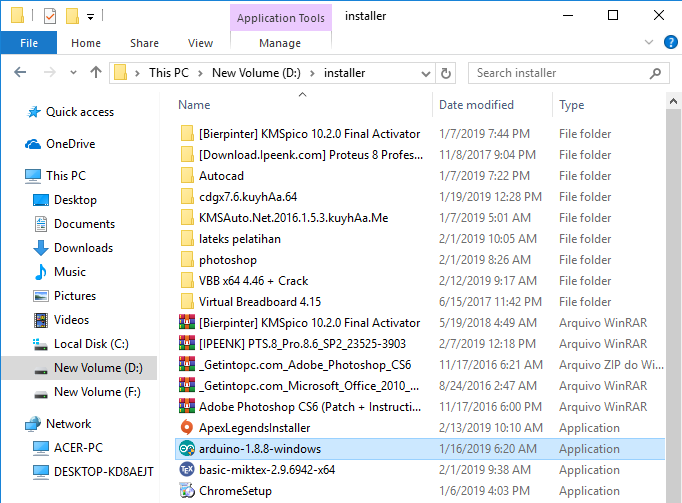
\includegraphics[width=.75\textwidth]{figures/IDE/installer.png}
            \caption{Ini adalah installer}\label{fig:installer}
            \end{figure}
        \item Maka akan tampil seperti gambar \ref{fig:agreement}
            \begin{figure}[!htbp]
            \centering
            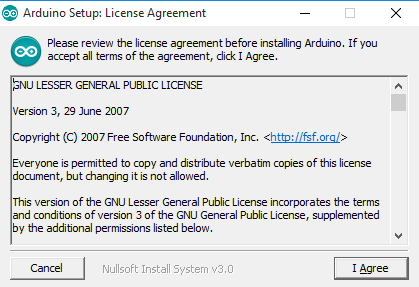
\includegraphics[width=.75\textwidth]{figures/IDE/agreement.png}
            \caption{Ini adalah Halaman Agreement}\label{fig:agreement}
            \end{figure}
        \item Pilih \textbf{Agree} maka akan muncul halaman \textit{Installation Options} seperti pada gambar \ref{fig:option}
            \begin{figure}[!htbp]
            \centering
            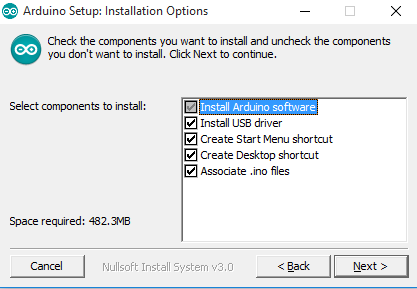
\includegraphics[width=.75\textwidth]{figures/IDE/option.png}
            \caption{Ini adalah Halaman Installation Options}\label{fig:option}
            \end{figure}
        \item Kemudian tekan tombol next, maka akan muncul halaman pemilihan direktori penyimpanan seperti pada gambar \ref{fig:dir}
            \begin{figure}[!htbp]
            \centering
            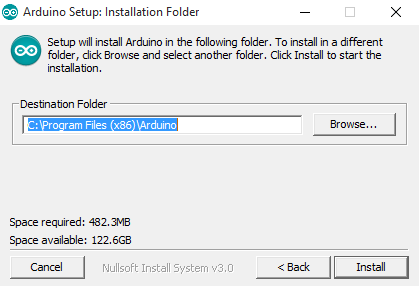
\includegraphics[width=.75\textwidth]{figures/IDE/dir.png}
            \caption{Ini adalah Halaman Pemilihan Direktori}\label{fig:dir}
            \end{figure}
        \item Kemudian tekan tombol install, maka proses installasi dimulai seperti pada gambar \ref{fig:installing}
            \begin{figure}[!htbp]
            \centering
            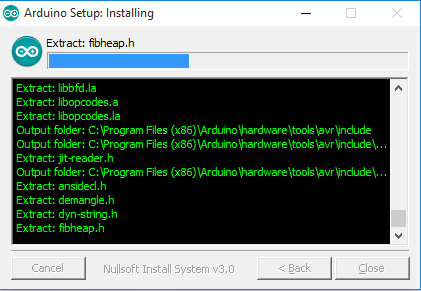
\includegraphics[width=.75\textwidth]{figures/IDE/installing.png}
            \caption{Ini adalah Proses Installasi IDE}\label{fig:installing}
            \end{figure}
        \item Proses installasi selesai, seperti pada gambar \ref{fig:complete}
            \begin{figure}[!htbp]
            \centering
            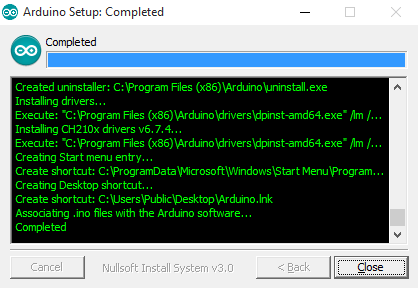
\includegraphics[width=.75\textwidth]{figures/IDE/complete.png}
            \caption{Ini adalah Proses Installasi Telah Selesai}\label{fig:complete}
            \end{figure}
        \end{enumerate}